\documentclass{article}
%\usepackage{geometry}
% \geometry{top = 1in, bottom = 1in, left = 1in, right = 1in}
\usepackage[top = 0.7in, bottom = 0.7in, left = 0.7in, right = 0.7in]{geometry}
\usepackage{amsmath,amssymb,amsthm,mathrsfs}
\usepackage{graphicx}
\usepackage{bm}
\usepackage{float}
\usepackage[font=footnotesize,labelfont=bf]{caption}

\usepackage{fancyhdr}
\pagestyle{fancy}
\rhead{\footnotesize {08/10/2012 ; MESA version 4278} }
\chead{\footnotesize {Authors: Jared Brooks, Lars Bildsten, Bill Paxton} }
\lhead{\footnotesize {mesa/star/test\_suite/multiple\_stars} }

\begin{document}
	
	\begin{center}
		\begin{Large}
		  \textbf{MULTIPLE STARS}\\
		\end{Large}
	\end{center}
	
        This test is to show how \texttt{MESA} can evolve multiple stars with separate inlists simultaneously.  Each star is evolved for the same amount of time, $1.5\times10^8$ years.  Therefore, if everything ran succesfully, the terminal output at the end of the run should read \texttt{``all stars have reached stopping age''}.\\

        Each star being computed in this test case has its own inlist.  The number of stars and the filenames of their inlists are set in \texttt{inlist\_multi\_stars\_job}, along with their stopping age (\texttt{stopping\_age = 1.5e8}).  The three inlists for this test are very similar.  The first inlist, \texttt{inlist1}, loads a pre-saved model, \texttt{m3ms.mod}, while the other two inlists load $Z=Z_\odot$ ZAMS models.  The only other difference is in the masses; inlists 1, 2, and 3 have masses 3 $M_\odot$, 3.1 $M_\odot$, and 3.2 $M_\odot$, respectively.   This setup allows users to evolve and compare similar stars simultaneously while still being able to change a wide set of parameters and controls for each star individually.\\

        Below is an HR-diagram showing the evolutionary tracks of all three stars (figure \ref{fig:1}).

        \begin{figure}[H]
                \centering
                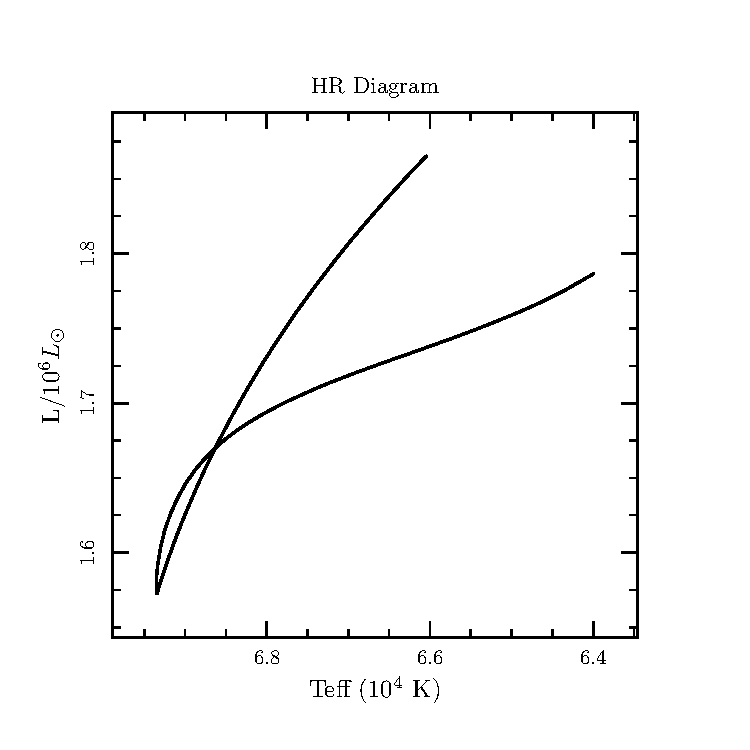
\includegraphics[width = 5in]{/Users/jaredbrooks/multiple_stars/plots_out/HR_Diagram.pdf}
                \caption{}
                \label{fig:1}
        \end{figure}

        \pagebreak

        The growth of the radius on the main sequence depends on the mass (Figure \ref{fig:2}), as does the rate of hydrogen consumption (Figure \ref{fig:3}).

        \begin{figure}[H]
                \begin{minipage}[b]{0.5\linewidth}
		       \centering
		       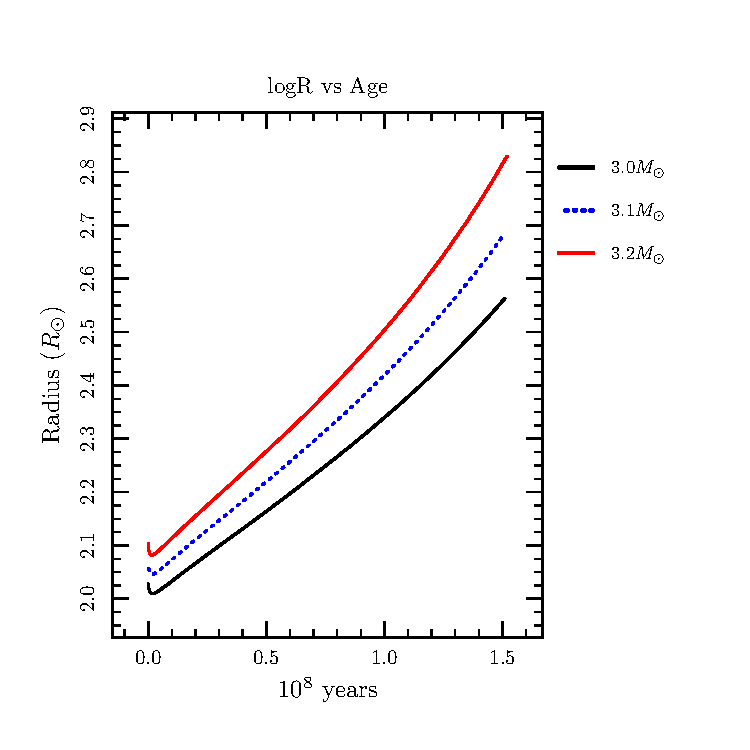
\includegraphics[width = 3.8in]{/Users/jaredbrooks/multiple_stars/plots_out/logR_vs_Age.pdf}
		       \caption{Radius evolution depends on mass}
		       \label{fig:2}
                \end{minipage}
                \hspace{0cm}
                \begin{minipage}[b]{0.5\linewidth}
                       \centering
                       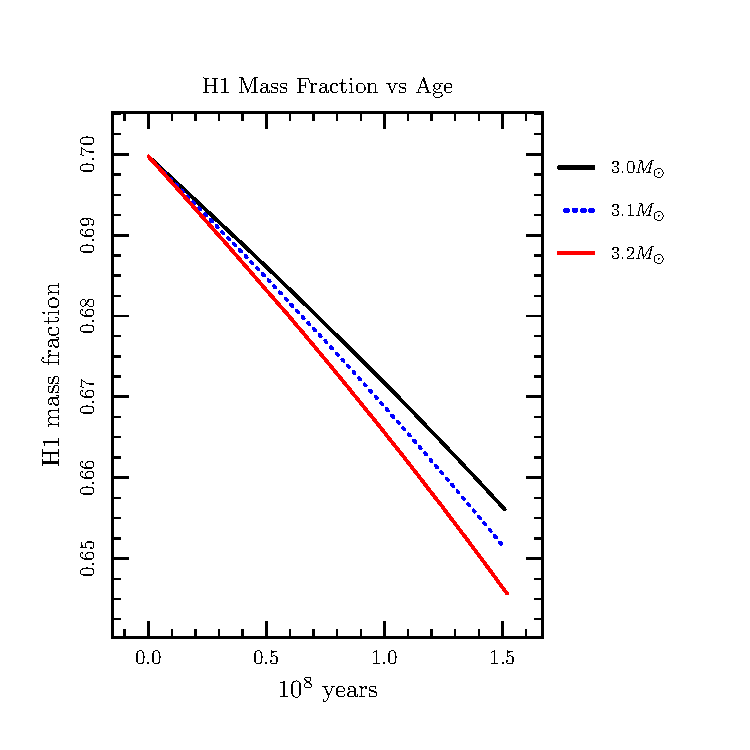
\includegraphics[width = 3.8in]{/Users/jaredbrooks/multiple_stars/plots_out/H_vs_Age.pdf}
                       \caption{Burning rate of Hydrogen depends on mass}
                       \label{fig:3}
                \end{minipage}
	\end{figure}


\end{document}


